\documentclass[a4paper]{article} 
\addtolength{\hoffset}{-2.25cm}
\addtolength{\textwidth}{4.5cm}
\addtolength{\voffset}{-3.25cm}
\addtolength{\textheight}{5cm}
\setlength{\parskip}{0pt}
\setlength{\parindent}{0in}

\usepackage[square,sort,comma,numbers]{natbib}
\usepackage{blindtext} % Package to generate dummy text
\usepackage{charter} % Use the Charter font
\usepackage[utf8]{inputenc} % Use UTF-8 encoding
\usepackage{microtype} % Slightly tweak font spacing for aesthetics
\usepackage{amsthm, amsmath, amssymb} % Mathematical typesetting
\usepackage{float} % Improved interface for floating objects
\usepackage{hyperref} % For hyperlinks in the PDF
\usepackage{graphicx, multicol} % Enhanced support for graphics
\usepackage{xcolor} % Driver-independent color extensions
\usepackage{pseudocode} % Environment for specifying algorithms in a natural way
\usepackage[mmddyy]{datetime} % Uses YEAR-MONTH-DAY format for dates

\usepackage{fancyhdr} % Headers and footers
\pagestyle{fancy} % All pages have headers and footers
\fancyhead{}\renewcommand{\headrulewidth}{0pt} % Blank out the default header
\fancyfoot[L]{} % Custom footer text
\fancyfoot[C]{} % Custom footer text
\fancyfoot[R]{\thepage} % Custom footer text
\newcommand{\note}[1]{\marginpar{\scriptsize \textcolor{red}{#1}}} % Enables comments in red on margin

\DeclareMathOperator*{\argmin}{arg\,min}

%----------------------------------------------------------------------------------------


%-------------------------------
%	TITLE VARIABLES (identify your work!)
%-------------------------------

\newcommand{\yourname}{Balthazar Neveu}
\newcommand{\youremail}{balthazarneveu@gmail.com}
\newcommand{\assignmentnumber}{1}

\begin{document}

%-------------------------------
%	TITLE SECTION (do not modify unless you really need to)
%-------------------------------
\fancyhead[C]{}
\hrule \medskip
\begin{minipage}{0.295\textwidth} 
\raggedright
\footnotesize
\yourname \hfill\\
\youremail
\end{minipage}
\begin{minipage}{0.4\textwidth} 
\centering 
\large 
Lab session \# \assignmentnumber\\ 
\normalsize 
ALTEGRAD 2023\\ 
\end{minipage}
\begin{minipage}{0.295\textwidth} 
\raggedleft
\today\hfill\\
\end{minipage}
\medskip\hrule 
\bigskip



%-------------------------------
%	ASSIGNMENT CONTENT (add your responses)
%-------------------------------
Introductory remarks regarding the jupyter notebook:
\begin{itemize}
    \item I wrote some tests for the encoder, decoder and attention modules to check that everything can be plugged in together correctly.
    \item I adopted the tensor notations [$L$, $N$, $H$] where $L$ is the sentence length, $N$ is the batch size and $H$ is a hidden dimension / feature dimension.
    \item I re-implemented a random sampling strategy based on the temperature parameter. Temperature=0 leads back to (argmax) greedy sampling which is what's used during training.
\end{itemize}

I wrote most of the report in the \textbf{old fashion way (manually)}, I explicitly mentioned in section 3 where ChatGPT4 was used for an assistance.

\section{Question 1: Greedy decoding strategy}

Greedy decoding strategy picks the translated token with the highest probability (argmax on the softmax of the logits getting out of the decoder).
There are naturally many other sentences possibilities which are not explored... but it is the least expensive solution in terms of computation cost:
\begin{itemize}
    \item It has the advantage of being fast since you predict the next word probabilities using a single inference of the recurrent decoder neural network.
    \item You can override (inplace) the decoder hidden state and context every time you go to the next word. 
\end{itemize}

There are a few solutions as mentioned in \cite{hugging_face_gen}
\begin{itemize}
\item  Exploring more solutions would naturally mean a higher computation cost. If you'd like to explore several possibilities, for each word you'd like to test, you'd have to run an inference to predict the next word (and in terms of memory, you'd need to keep a copy of the hidden states). This would be quite heavy and leads to exponential combinations (the word decision tree quickly becomes huge). In beam search you may keep only a fixed amount of combinations.
\item  Performing random sampling. Instead of taking the most probable word, why not sampling randomly from the predicted distribution. 
This may lead to unexpected results as we add a bit of randomness in the process. \ref{fig:random_sampling}
\end{itemize}
Finally, despite trying a simple different sampling strategy, I still cannot improve the translation quality. I think it is hard to tell whether or not the sampling strategy impacts the final results as the overall model quality seems pretty low. See Section 2. for more details about this.

\begin{figure}[ht]
    \centering
    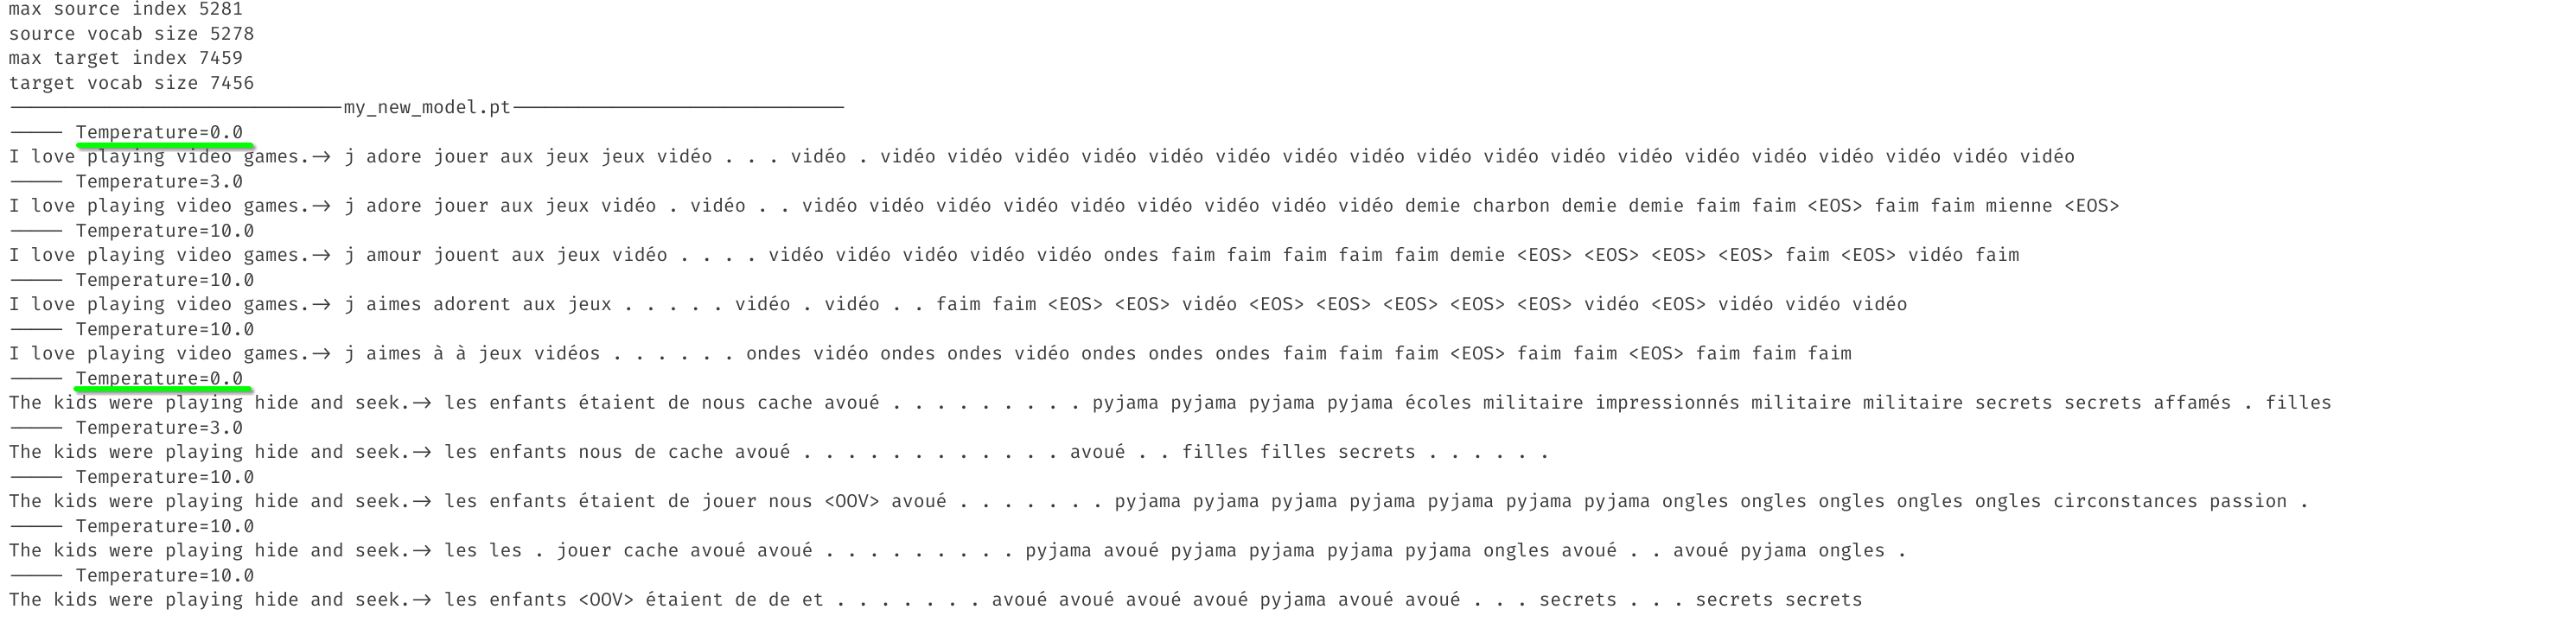
\includegraphics[width=0.5\linewidth]{figures/temperature_sampling.png}
    \caption{Random sampling on the distribution using the temperature parameter. Temperature = 0 is equivalent to the argmax sampling.}
    \label{fig:random_sampling}
\end{figure}



\section{Question 2: Issues with the translations}
Overall, my personal subjective evaluation is that the translation quality is not so great.
Before going into the overall analysis of some examples and try to describe complex phenomenon, it is necessary to point out some of the caveats of the current training... Mostly due to lack of time.
\begin{itemize}
\item \textbf{Creating baselines}: First step would have been to train a simple N-gram model on the chosen dataset to have a baseline. Second step would have been to train the seq2seq RNN without attention to get another baseline.
\item \textbf{Hyper parameters have not been tweaked}. A learning rate schedule would have been nice (e.g after 80 epochs, learning rate should have been decreased to maybe keep on going).
\item \textbf{Slight hints of start of overfitting}: It looks like during my training with a learning rate of $10^{-3}$ and all default parameters provided, the test got to a plateau but the train loss kept on decreasing, meaning a slight risk of overfitting on the training set (the test loss did not go up though so it's not an explicit sing of overfit, just a hint that the network is not learning to generalize as much as in the begining.)\textit{ Memorizing language patterns may be a good idea, but not training sentences word by word.}
\end{itemize}

\begin{figure}[ht]
    \centering
	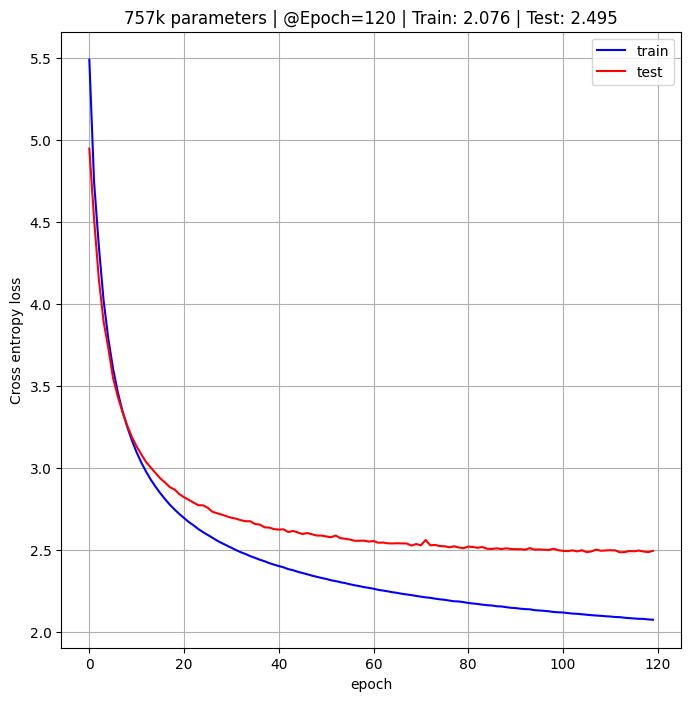
\includegraphics[width=.6\textwidth]{figures/training_curve.png}
	\caption{Training metrics with default parameters ($lr=10^{-3}$ , $batch\;size=128$) \label{fig:metric}}
\end{figure}

Here are some key design points which may also have been re-considered for future work.
\begin{itemize}
\item \textbf{Shallow network}: The encoder tries to build a hidden state which compresses the whole sentence meaning into a single vector. Since there's only a single GRU (no a deep stack of GRU) in the stack, the encoder is doing pretty simple operations by making temporal combinations of the word embeddings thanks to the GRU. The lack of depth (deep means we have many linear weights multiplication followed by non linearities) forces the encoder to make basic representations.
\item There are 757k parameters in the model, most of the parameters are used to build the embeddings(Source embeddings  211k, 
Target embedding  298k = in total 509k parameters are basically a look up table to go from words to floating point vectors. Decoder prediction  has 223k parameters to project back the hidden to probabilities (basically a reverse lookup table). To learn the structure of sentences and language, the GRU has a few parameters to learn which feature dimension to focus on (memorize) to create a sentence summary vector.
\item The source sentence is analyzed in a causal manner in the encoder. The GRU cannot look backwards (uni-directional). We'll come back to that point in Section 4.
\item The "alignment" mechanism performs weighted sums of the current decoded hidden state and all source encoded vectors. With linear combinations and a $tanh$ function, \textbf{it does not seem straightforward that similarities between words can be computed}. The cosine distance/dot product or the L2 distance between target hidden state and source hidden vectors sounds much more appropriate... and this is what ended up being used in Transformers\cite{vaswani2017attention_transformer} obviously.
\end{itemize}



Overall, when looking at the translation results, it is difficult to decouple issues which may come from true limitations (inherent translation task challenges, archictecture design) or what comes from the short amount of time spent on polishing the training (basically not picking low hanging fruits that a machine learning practitioner would usually try with a bit more time).


\begin{verbatim}
She eats a pizza, her friend opens a beer and her baby is sleeping. 
-> elle mange une pizza , l son ami de une la et son père père .
\end{verbatim}


Let's still try to analyze some translation results as best as we can.
\begin{itemize}
\item Over-translation: repeated words (père, père)
\item Under-translation: missed words (bière)
\item Hallucination: translated sentences which almost make sense but do not match the source content ("et son père" does not match with the source sentence but still sounds alright.
\item Difficulty to capture long range dependencies (difficult to illustrate here: "her" in "her baby" refers to the woman eating a pizza which was at the begining of the sentence - not to a man "père"...).
\end{itemize}


\begin{center}
  $\ast$~$\ast$~$\ast$
\end{center}


\textbf{Greedy sampling is performed both during training time and inference}. This is a nice point as there is no gap between training and inference. But the decoder is not trained with the groundtruth previous words (assuming the past translation is perfect). This probably makes the task even more difficult e.g. anytime the model makes a mistake, it will be almost impossible to learn the rest of the translation. We probably remove a bunch of learning signal for this reason.

\begin{verbatim}
The cat fell asleep in front of the fireplace 
-> le chat s est en du du pression peigne peigne cheminée portail
portail portail portail portail portail portail portail indépendant
oiseaux oiseaux oiseaux oiseaux oiseaux oiseaux oiseaux oiseaux
oiseaux oiseaux
\end{verbatim}
As soon as the translated words start to mess up, the decoder ends up in a similar "bad" situation as seen during training. But it probably never got out of that trap at training time either.


\begin{verbatim}
I have blue eyes. -> j ai les yeux bleus bleus .
\end{verbatim}

We get a some repeated words (over-translation). An easy pragmatic way to solve this would be to manually discard these repetitions afterward. But the interesting fact is that the model creates these repeated words.\\
Although there's a no explicit way to debug /explain this issue, \textit{a good heuristic which could be used is that a word which has already been translated shall get less attention than the other remaining words.}
In the sentence "I have blue eyes.", bleus shall attend to "eyes" to know whether it's a plural or singular. So keep in mind that totally discarding the word "eye" after it's been translated may not be an ideal idea. Still, if a mechanism is built in the end to end training process to perform this task, it seems like a good idea.\\


This is the idea behind the Coverage Mechanism proposed in \cite{modeling_coverage}.\\
\textit{I do not pretend to fully understand the implementation details, but below is the general idea behind the coverage mechanism.}\\
There is a direct way to keep track of attention history. For every decoder time step, an accumulated attention weight is maintained, which stores the sum of attention weights over all previous decoder time steps for each source word. An concrete example: in \ref{fig:attention}, you'd progressively sum vertically. This accumulated weight is then used in conjunction with the current attention distribution to penalize attending to source words that have already been attended to. The idea is to guide the attention mechanism to focus on unattended or less-attended parts of the source sentence. At training time, this would be implemented as an extra penalty term added to the Cross Entropy Loss we used in the lab session. 
The under-translation/missing word issue seems to be solvable in the same fashion. In \ref{fig:attention}, we can visualize that "Red" has almost not been matched to any translated word (the column is a bit darker than some other columns like "wine" or "open").

\newpage
\section{Question 3: Alignment visualization}

\begin{figure}[ht]
    \centering
	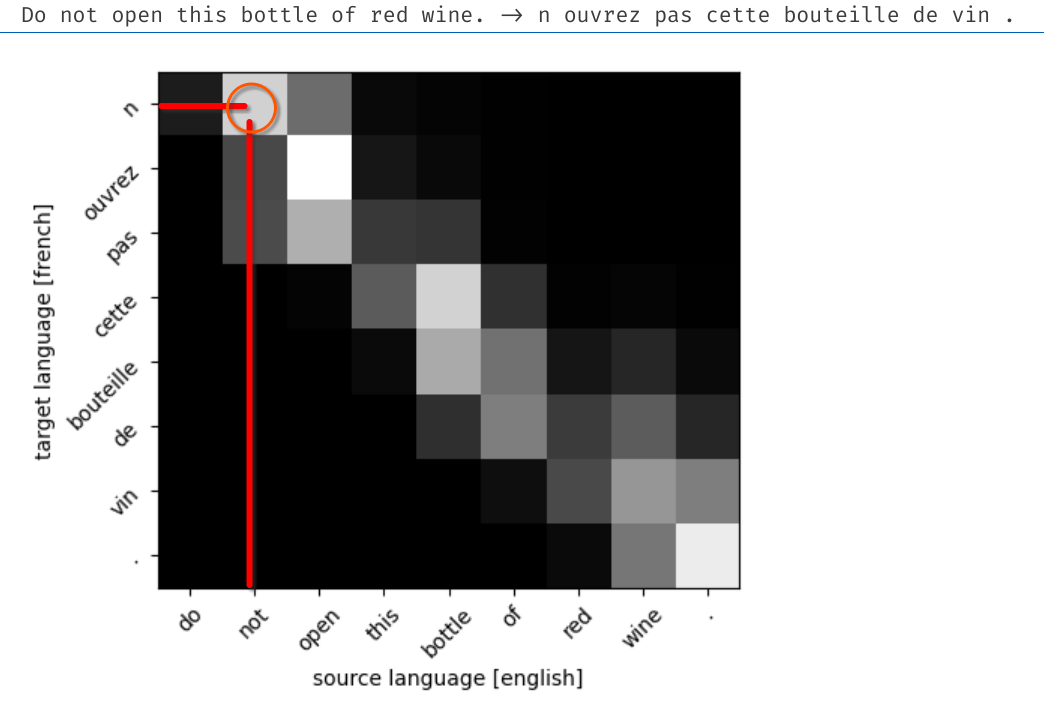
\includegraphics[width=.8\textwidth]{figures/bottle_of_wine.png}
	\caption{Alignment scores captured on the sentence label. Each row describes a translated word in the target model. The sum of all score elements over a row shall be 1 to be able to perform the weighted sum (this is granted by the softmax).\label{fig:attention}}
\end{figure}

Figure \ref{fig:attention}  ilustrates a difficult word inversion captured by a high score between french "n'" and the second sentence word in english "not". Let's take the first row, french word "n' " was compared to the 9 words of the source sentence.
We can see that the most relevant english word was "not" according to the score. Which wasn't the first word of the sentence. A naive word by word translation would have led to "faire ne ouvrir"... here the alignment/attention mechanism most helped the first translated word to look a bit ahead in the source sentence. \\
Having the ability to \textbf{perform word inversion during decoding is a mandatory component in machine translation.}\\ \\
On the other hand, we can also see one of the drawback of the current alignment mechanism: some words have been skipped. Where we would have expected "rouge" to be, "vin" was translated instead... This is pretty straightforward to explain, the score mostly matched with the "wine" word but the "red" word got less attention (it was clearly forgotten here). We mentioned the under translation phenomenon in the previous section, here it seems like we almost get an explicit explanation of the phenomenon.\\


\begin{figure}[H]
    \centering
	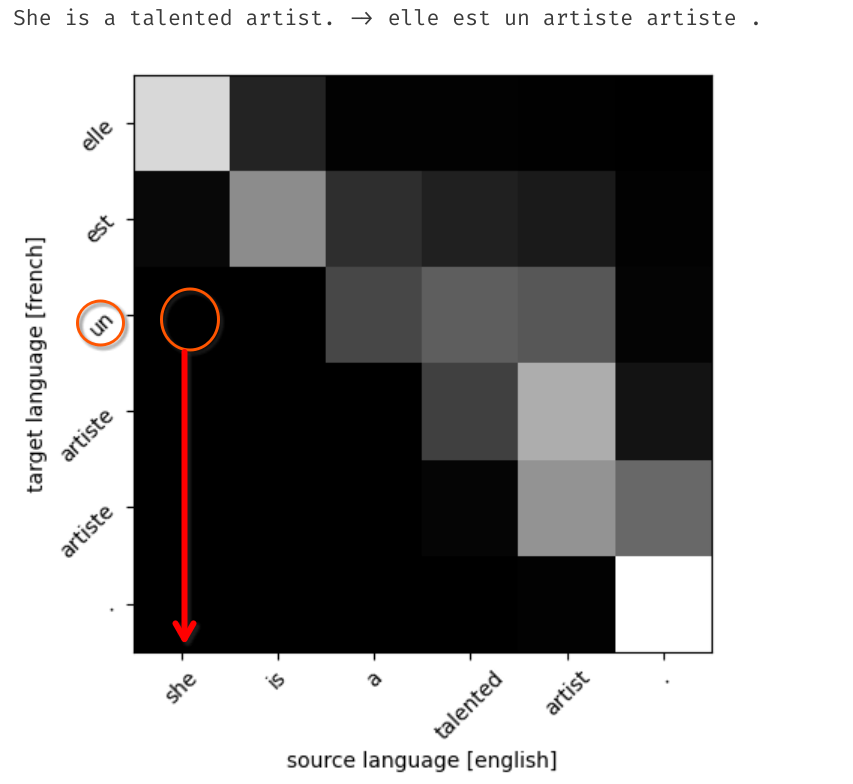
\includegraphics[width=.6\textwidth]{figures/gender_issue.png}
	\caption{Gender inference fails.\label{fig:Gender}}
\end{figure}

\textit{Note: The following list was inpsired with an assistance from ChatGPT 4}. Examples were tested with the pretrained model. (refer to the examples in the notebook for full content).\\
Here's a list of difficult translations phenomenon where attention is a key ingredient for success.
\begin{itemize}
\item \textbf{Adjective-Noun Inversion}: \textit{English: "blue car" / French: "voiture bleue" (literally: "car blue")}
\item \textbf{Verb-Subject Inversion in Questions}: \textit{English: "Are you coming?" / French: "Viens-tu?" (literally: "Come-you?")}
\item \textbf{Gender and Number Agreement}: \textit{English: "A car" / French: "Une voiture" (feminine)} French nouns have gender (masculine or feminine), which affects the form of adjectives, articles, and sometimes verbs. English doesn't have this gender distinction for inanimate objects. A failure case is illustrated in \ref{fig:Gender}
\item \textbf{T-V Distinction}: French, like many other languages, has a distinction between formal and informal address ("vous" vs. "tu"). English uses "you" for both. A failure is illustrated in \ref{fig:T-V distinction}

\begin{figure}[h!]
    \centering
	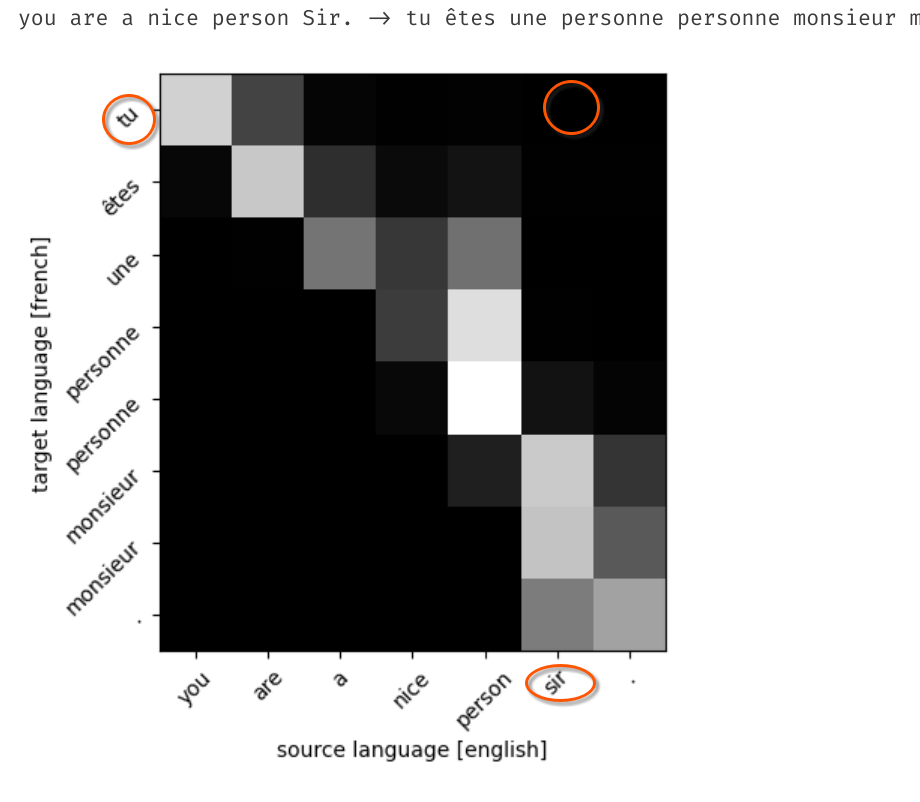
\includegraphics[width=.6\textwidth]{figures/Tu_Vous.png}
	\caption{T-V distinction fails. "Tu" shall have looked at the last source sentence word "Sir" to disambiguate.  But that score circles in red is close to 0\label{fig:T-V distinction}}
\end{figure}

\item \textbf{Subjunctive Mood}:
French: "Il faut que tu viennes" (It is necessary that you come)
English might simply say: "You need to come."  The subjunctive mood is used more frequently in French than in English. It can be challenging to translate accurately because its use in English is more limited and often context-specific.
\item  \textbf{Negation}: English: "I don't know" / French: "Je ne sais pas" (literally: "I no know not") \textit{French typically uses a two-part negation.} \ref{fig:Negation}
\item  \textbf{Placement of Adverbs:} English: "I often eat apples"
French: "Je mange souvent des pommes" (literally: "I eat often apples") \textit{The placement of adverbs can vary between English and French.}
\item \textbf{Prepositions}: English: "I am good at maths" / French: "Je suis bon en maths" (literally: "I am good in maths") \textit{The use and choice of prepositions can differ significantly between English and French.}
\end{itemize}





\begin{figure}[h!]
    \centering
	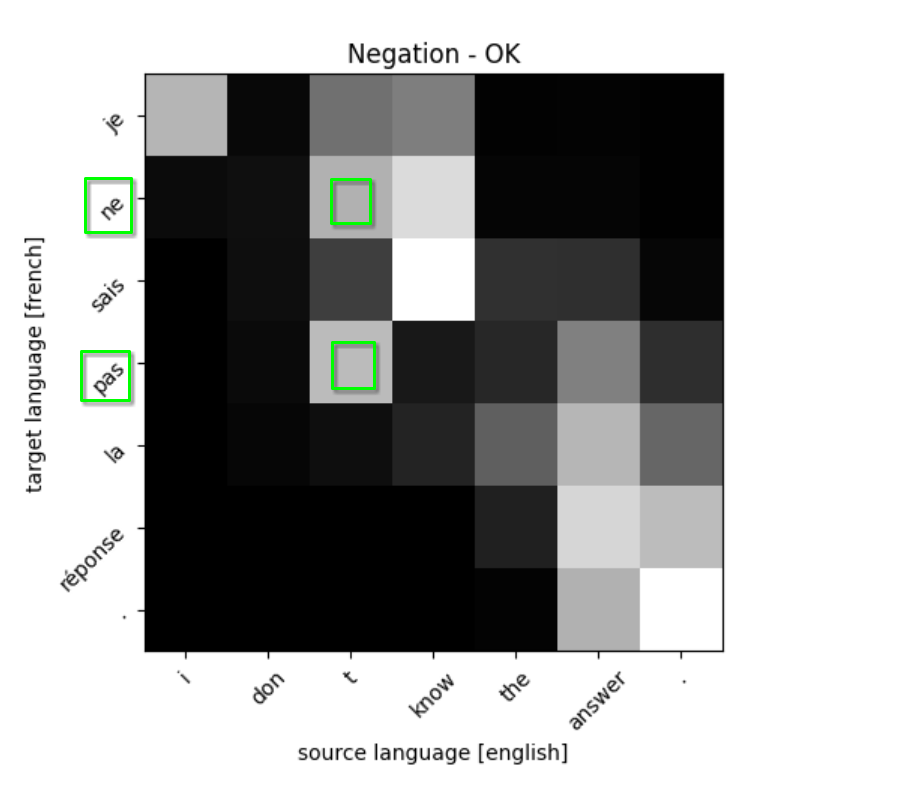
\includegraphics[width=.5\textwidth]{figures/negation.png}
	\caption{Negation : Je ne sais pas la réponse, ne and "pas" both had scores matching that abrreviated t = not  \label{fig:Negation}}
\end{figure}

\newpage
\section{Question 4: Polysemy}
Note: \textit{ChatGPT4 was powerful enough to retrieve the concept "Polysemy" when prompted with the example. incredible} \\

\begin{verbatim}
I did not mean to hurt you
She is so mean
\end{verbatim}


\textbf{Polysemy} : The same word may have different meaning depending on the context. 
In the first case, "mean" is a verb. In the second case "mean" is an adjective. But both are written the same in english and \textbf{will get the same embedding vector in the encoder}.



\textbf{TL/DR}: Here are some key ingredients to address polysemy and general ideas to improve
\begin{itemize}
\item \textbf{Attend the whole sequence}: For each word/token in the source sentence, looking at the whole source sentence is important. Self attention looks at the whole sentence  \cite{vaswani2017attention_transformer} (bidirectional in the encoder - but decoder is unidirectional), \textbf{Bidirectional} RNN as proposed in ElMo use 2 passes \cite{context_rep} . Caveat: in our lab, we used uni-directional GRU, this is a potential improvement to consider).
\item \textbf{Stacking several layers of linearity/non linearities} allows creating powerful representations. Working with a single linear word embedding + a single  GRU (no stacks) like we did in the lab is probably not enough.
\item \textbf{Next word prediction in the source language.} Working on the encoder itself can be decoupled from the translation task. \textbf{Powerful representations can be created by only looking at a corpus of the source language} with much more data available. Next word prediction allows pretraining the encoder (so called unsupervised training as you don't need pairs of labeled data for instance). Note: next word prediction does not allow the attention to be bi-directional. BERT \cite{bert} pretrains on the masked word prediction task which allows the attention to be bidirectional (only at the encoder level).
\end{itemize}



\begin{center}
  $\ast$~$\ast$~$\ast$
\end{center}

\textbf{Disclaimer} I wrote the following paragraph with my own reflections and read BERT \cite{bert} and ElMO \cite{context_rep} only at the end, just to try to push my reflection as far as I could go.  Writing this answer sort of helped me understand some of the Transformers design choice which I took basically from granted.

\begin{center}
  $\ast$
\end{center}


One may expect that some components of the feature vectors for each word to specialize in describing higher level concepts (e.g. what gender it represents or the type of word like adjective/noun/verb). The default embedding for "mean" would have say 0.5 for the adjective dimension, 0.5 for the "is it a verb" dimensions. \\
Example: we have 30 dimensions in the encoder hidden state, let's assume that dimension 28 for instance is dedicated to describing how likely a given word is a verb, and the 13th component is dedicated to describe how likely a word is an adjective . 
The recurrence (GRU) may help to refine the knowledge of the "type of word". In the second translation case (she is so mean): the encoder may refine the 28th component of the hidden state to be near 0 and the 13th component to be closer to 1. This is pure intuition and interpretation of the mechanism of the neural network, things may not work that way in practice unfortunately.

Unfortunately:
\begin{itemize}
\item In the current setting, we're hopping that the encoder uses the temporal aspect of the gated recurrent unit (GRU) to compute a context in the input sentence (decide what to memorize). Issue is that there are not many parameters in the GRU and that the GRU only accesses previous elements. It is a causal recurrent unit.
\item This relevant piece information (adjective/verb) may be lost in the middle of many other significant embedding dimensions (like simply embedding the meaning of the word, not grammar properties or more abstract thing) as this is a translation task.
\end{itemize}



Several ideas appear before we'd start considering self-attention in the source language:
\begin{itemize}
\item Chain several layers on linear/non linear so a lot more complex representations can be created and hope that each GRU start to specify in given subtasks. In ElMO \cite{context_rep}, they stacked 2 bidirectional LSTM.
\item Chunk hidden feature into several smaller vectors and feed to several GRU in parallel. Although there is no explicit way to teach the network to specialize its feature into learning specific linguistic concepts, it seems like forcing to learn independent language properties (like grammar, gender, word type etc...) is worth trying to improve performances. This is a similar idea to MHA (multi-head attention) which also seems to be one of the ingredient of the Transformer: it ends up with specialized features (intuition  = specialized in analyzing grammar or singular/plural features).
\end{itemize}

\begin{center}
  $\ast$~$\ast$~$\ast$
\end{center}

A simple remark: \textbf{why would we wait for the decoding step to start doing implicit sentence analyzis?}. After all, we don't need the translation task to be able to analyze the sentence in the source language.
\begin{itemize}
    \item We can think as the encoder outside of the "translation" task and simply stay in a "unsupervised" next word prediction task in the source language. This would help to build as a pre-training step hidden vector representation which are more powerful than then ones in the translation supervision settings. Reason is simple: we'd be able to get much more data as we don't need pairs of translated sentences. Just a raw french or english corpus for instance.
    \item The attention mechanism looks like a great idea to take context into account... Why restricting it to the cross language attention? Why not performing self attention on the source domain? (and actually be able to replace the RNN). It became sort of a standard principle in the Transformer paper \cite{vaswani2017attention_transformer}: using \textbf{self attention}.
\end{itemize}

\begin{center}
  $\ast$~$\ast$~$\ast$
\end{center}



%------------------------------------------------

\bibliographystyle{plain}
\bibliography{references} % citation records are in the references.bib document

\end{document}